
\section{Relevant Results}


\begin{figure}[h!]
    \centering
    \begin{minipage}{0.5\textwidth}
        \centering
        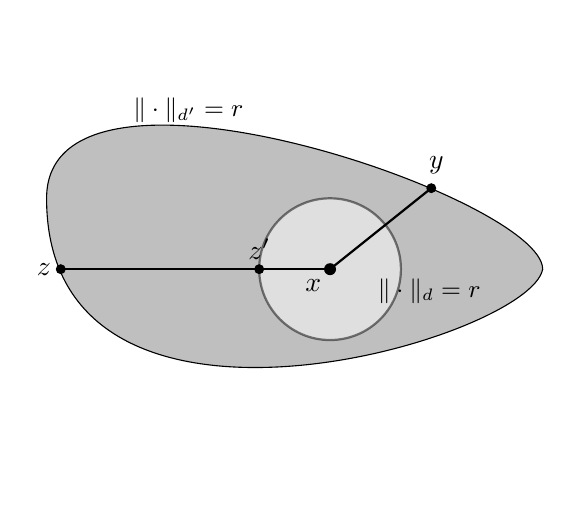
\begin{tikzpicture}[scale=1.8]
            % Rotate and draw the bean shape
            \begin{scope}[local bounding box=C, shift={(0,0)}, rotate=90] 
                \draw[fill=gray!50] 
                    (0,-1.5) .. controls +(170:.5) and +(180:2) ..
                    (.5,2) .. controls +(0:1.2) and +(0:.5) .. cycle;
            \end{scope}

            % Draw the inner circle
            \draw[thick,fill=white!50,opacity=.5] (0,0) circle (.5);

            % Draw the center of the circle
            \fill (0,0) circle (1.2pt);

            % Draw two lines intersecting the outer shape from the center of the circle
            \draw[thick] (0,0) -- (1.5/2.1,1.2/2.1);
            \draw[thick] (0,0) -- (-1.9,0);

            % Draw the points on the longer segment between the circle and the outer shape
            \fill (-0.5,0) circle (1pt);
            \fill (-1.9,0) circle (1pt);
            \fill (1.5/2.1,1.2/2.1) circle (1pt);

            % Label the inner circle
            \node[below] at (0.7,0) {\small{$\|\cdot\|_d = r$}};

            % Label the outer shape
            \node at (-2.5/2.5,2.8/2.5) {\small{$\|\cdot\|_{d'} = r$}};

            % Label the center
            \node at (-0.2/1.7,-0.2/1.7) {$x$};

            % Label the intersections of the line segments with the outer shape
            \node[above] at (1.5/2,1.2/2) {$y$};
            \node[left] at (-1.9,0) {$z$};

            % Label the point on the longer segment
            \node[above] at (-.5,0) {$z'$};
        \end{tikzpicture}
        
        %\label{fig:bean_shape}
    \end{minipage}\hfill
    \begin{minipage}{0.5\textwidth}
        \centering
        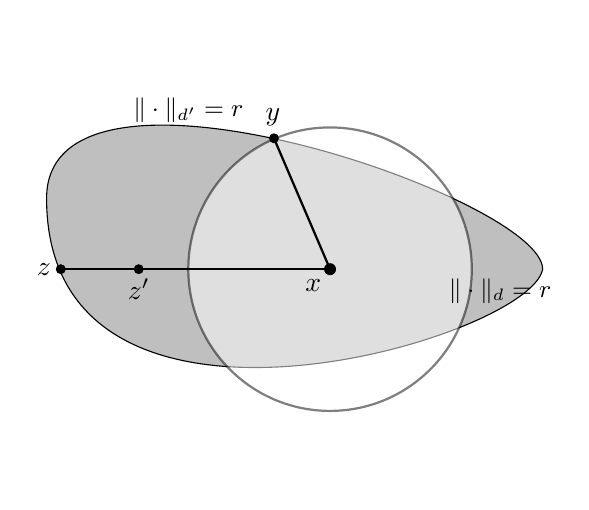
\begin{tikzpicture}[scale=1.8]
            % Rotate and draw the bean shape
            \begin{scope}[local bounding box=C, shift={(0,0)}, rotate=90] 
                \draw[fill=gray!50] 
                    (0,-1.5) .. controls +(170:.5) and +(180:2) ..
                    (.5,2) .. controls +(0:1.2) and +(0:.5) .. cycle;
            \end{scope}

            % Draw the bigger inner circle
            \draw[thick,fill=white!50,opacity=.5] (0,0) circle (1);

            % Draw the center of the circle
            \fill (0,0) circle (1.2pt);

            % Draw two lines intersecting the outer shape from the center of the circle
            \draw[thick] (0,0) -- (-1.5/3.79,3.5/3.79);
            \draw[thick] (0,0) -- (-1.9,0);

            % Draw the points on the longer segment between the circle and the outer shape
            \fill (-1.35,0) circle (1pt);
            \fill (-1.9,0) circle (1pt);
            \fill (-1.5/3.79,3.5/3.79) circle (1pt);

            % Label the inner circle
            \node[below] at (1.2,0) {\small{$\|\cdot\|_d = r$}};

            % Label the outer shape
            \node at (-2.5/2.5,2.8/2.5) {\small{$\|\cdot\|_{d'} = r$}};

            % Label the center
            \node at (-0.2/1.7,-0.2/1.7) {$x$};

            % Label the intersections of the line segments with the outer shape
            \node[above] at (-1.5/3.72,3.5/3.72) {$y$};
            \node[left] at (-1.9,0) {$z$};

            % Label the point on the longer segment
            \node[below] at (-1.35,0) {$z'$};
        \end{tikzpicture}
        %\caption{A bean-shaped diagram with a larger circle intersecting the outer shape}
        %\label{fig:bean_shape_bigger_circle}
    \end{minipage}
    \caption{Relative scaling of $r$-balls of norms $||\cdot||_d$ and $||\cdot||_{d'}$.}
    \label{fig:norm}
\end{figure}

\begin{theorem}
    Let $\cB$ be a complete normable vector space. Let $$\mathfrak{B}:= \curlybracket{d: \cB \times \cB \to \reals_{+}\,|\, \forall x,x' \in \cB, d(x, x') = ||x-x'|| \textnormal{ for a fixed norm on } \cB. }$$ 
    Using triplet constraints, a teacher can specify a target metric $d \in \mathfrak{B}$ up to linear scaling relation $\sim_R$. 
    %be a real normed vector space with the norm $||\cdot||$. Then, we can obliviously teach the norm up to 
\end{theorem}
\begin{proof}
Let $d$ and $d'$ be two norm induced metrics not related up to linear scaling but they satisfy the same triplet relation on any $x,y,z \in \cB$. Now, for a positive scalar $r > 0$ the closed balls $\overline{B_{d}(x,r)}$ and $\overline{B_{d'}(x,r)}$. Since $d$ and $d'$ are not related up to linear scaling, there exists a scalar $r > 0$ and a point $x$ such that the closed balls of radius $r$ centered at $x$ are scaled different, i.e there exists $y,z$ such that $\frac{d(x,y)}{d(x,z)} \neq \frac{d'(x,y)}{d'(x,z)}$.

Now, there are two possibilities: i) $\partial{B_{d}(x,r)} \cap \partial{B_{d'}(x,r)} \neq \emptyset$ or ii) $\partial{B_{d}(x,r)} \cap \partial{B_{d'}(x,r)} = \emptyset$.

We will show a contradiction for $i)$, whereas the contradiction for $ii)$ follows from a simple manipulation using $i)$. 

(consider right diagram in \figref{fig:norm})
If $\partial{B_{d}(x,r)} \cap \partial{B_{d'}(x,r)} \neq \emptyset$ there exists points (wlog) $y,z$ such that $y \in \partial{B_{d}(x,r)} \cap \partial{B_{d'}(x,r)}$ but $z \in \overline{B_{d'}(x,r)} \setminus \overline{B_{d}(x,r)}$. Thus, note that $d(x,z) > r$ but $d(x,y) \le r$. Now, there exists scalar $1> t > 0$ such that $z' := t x + (1-t) z \in \overline{B_{d'}(x,r)} \setminus \partial{B_{d}(x,r)}$, but then $d(x,z') > r$. Furthermore, $d'(x,z') > r$. Thus, for the points $x,y,z'$ we have
\begin{align*}
    d(x,y) = r < d(x,z') \textnormal{ but } d'(x,y) = r > d'(x,z')
\end{align*}
But this is contrary to the assumption that $d$ and $d'$ respect all triplet comparisons.

(consider left diagram in \figref{fig:norm}) If $\partial{B_{d}(x,r)} \cap \partial{B_{d'}(x,r)} = \emptyset$ there exists points (wlog) $y,z \in \partial{B_{d'}(x,r)} \setminus \overline{B_{d}(x,r)}$. Thus, note that $d'(x,z) = d'(x,y) = r$. Now, there exists scalar $1> t > 0$ such that $z' := t x + (1-t) z \in \partial{B_{d}(x,r)}$, but then $d(x,z') = r$. Furthermore, $d'(x,z') < r$. Thus, for the points $x,y,z'$ we have
\begin{align*}
    d(x,y) > r = d'(x,y) \textnormal{ but } d(x,z') = r < d'(x,z')
\end{align*}
Thus, even in this case, there exists a triplet comparison on which $d$ and $d'$ differ.

Hence, if $d$ and $d'$ are not related up to linear scaling, triplet comparisons can specify the same.


\end{proof}

\begin{theorem}
    For $c$-approximte teaching, there exists a set of size $2d$ for oblivious teaching.
\end{theorem}

\sanjoy{Some questions:}
\begin{enumerate}
\item \sanjoy{Triplets specify a Mahalanobis distance function upto a constant multiple. Is this true of any norm?} \akash{True} \sanjoy{Can you put in the proof?}
\item \sanjoy{Let's consider a $c$-approximate version of the learning problem, for $c \geq 1$. Let $d_M$ be the Mahalanobis distance induced by matrix $M$. If the target is $M^*$ then the $c$-approximate problem is to find a matrix $M \succeq 0$ such that $d_M(x,x') \geq d_M(x,x'')$ whenever $d_{M^*}(x,x') \geq c \cdot d_{M^*}(x,x'')$. What is the sample complexity of this relaxed learning objective? Here's one possible notion: we say $M, M'$ are $c$-close if there exists $\lambda > 0$ such that
$$ \frac{1}{c} \leq \lambda \cdot \frac{u^T M' u}{u^T M u} \leq c$$
for all $u \neq 0$.}
\item \sanjoy{In the setting where triplets need to be chosen from some pre-defined pool of points, it may not be possible to use multiples of the points (they may not correspond to real examples). In such cases, what is a good strategy for choosing triplets?}
\item \sanjoy{One setting of interest is the high- or infinite-dimensional regime, where the learner would need to choose a distance function based on just a few features. What are reasonable learning strategies in such cases?}
\end{enumerate}

\section{Oblivious teaching of Mahalanobis distance metric}

In this section, we will discuss oblivious teaching of the Mahalanobis distance metric. We assume that the metric model, denoted as $\cM_{\mathsf{maha}}$, contains Mahalanobis distance metrics as described below:
\begin{align*}
    \cM_{\mathsf{maha}} = \curlybracket{d: \cX \times \cX \to \reals_{+}\,|\, \exists M \in \textsf{symm}_{+}(\reals^d), s.t.\, d = d_M \textit{ as shown in }\eqnref{eq: maha} }
\end{align*}
The interaction protocol is shown in \algoref{alg: maha}. 

\begin{algorithm}[H]
\caption{Teaching a mahalanobis distance metric}
\label{alg: maha}
\textbf{Given}: Input space $\cX \subset \reals^d$, metric model $\cM_{\mathsf{maha}}$\\
\vspace{1mm}
\textit{In batch setting:}\vspace{1mm}
\begin{enumerate}
    \item teacher picks triplets $\cT(\cX,d_{M^*}) =$ $\curlybracket{(x,y,z) \in \cX^3 \,|\, (x-y)^{\top}M^*(x-y) \ge (x-z)^{\top}M^*(x-z)}$
    \item learner receives $\cT$; and obliviously picks a metric $d \in \cM_{\mathsf{maha}}$ as per \eqnref{eq: sol}
\end{enumerate}
\end{algorithm}

First, we note that using triplet comparisons alone learner can't find a fixed target matrix $M^*$ because for any $\lambda > 0$ and $(x,y,z) \in \cX^3$
\begin{align*}
    (x-y)^{\top}M^*(x-y) \ge (x-z)^{\top}M^*(x-z) \implies (x-y)^{\top}(\lambda M^*)(x-y) \ge (x-z)^{\top}(\lambda M^*)(x-z)
\end{align*}

Thus, we can only hope to find $d_{M^*}$, alternatively $M^*$ up to a positive linear scaling. Thus, we define a linear scaling relation $\sim_{R_l}$ on the space $\cM_{\mathsf{maha}}$ as follows:
\begin{align*}
   \textnormal{for any } d_M, d_{M'} \in \cM_{\mathsf{maha}}, d_M \sim_{R_l} d_{M'} \textnormal{ iff }  M = \gamma \cdot M' \textnormal{ for } \gamma > 0
\end{align*}
In the rest of the discussion, we study the oblivious teaching complexity of metric learning of mahalanobis distance metric wrt to the linear scaling relation $\sim_{R_l}$. 

In the rest of the section, we follow the notations as mentioned below:
%\sanjoy{I didn't get far in sections 2-3 because of high-level issues (see my comments). Can you fix these things and then I will go through these two sections more carefully.}
%\sanjoy{What is the formal model -- what problem is being solved?}
\paragraph{Notations:} For a given matrix $M \in \reals^{d\times d}$ and indices $i,j \in \bracket{d}$ $M_{ij}$ denotes the entry of $M$ at $ith$ row and $jth$ column. Matrices are denoted as $M,M',N$. Unless stated otherwise, a target matrix (for teaching a mahalanobis metric) is denoted as $M^*$. We denote that null set of a matrix $M$, i.e. $\curlybracket{x \in \reals^d\,|\, Mx = 0}$, as $\nul{M}$.
For a matrix, we denote its eigenvalues as $\gamma,\lambda, \gamma_i$ or $\lambda_i$ and its eigenvectors (orthogonal vectors) as $\mu_i ,u_i$ or $v_i$. We define the element-wise product of two matrices $M,M'$ via an inner product $\inner{M', M} := \sum_{i,j} M'_{ij}M_{ij}$. 
We denote vectors in $\reals^d$ as $x,y$ or $z$.
Note, for any $x \in \reals^d$ $\inner{xx^{\top}, M} = x^{\top}Mx$. For ease of notation, we also write the inner product as $M \idot M'$.

We denote the space of symmetric matrices in $\reals^{d \times d}$ as $\symm$, and similarly the space of symmetric, positive semi-definite matrices as $\symmp$.
Since the space of matrices on $\reals^{d\times d}$ is isomorphic to the Euclidean vector space $\reals^{d^2}$ for any matrix $M$ we also call it a vector identified as an element of $\reals^{d^2}$. We say two matrices $M,M'$ are \tt{orthogonal}, denoted as $M \bot M'$, if $M \idot M' = 0$. For a set of vectors/matrices $\cC \subset \reals^{d\times d}$, the subspace induced by the elements in $\cC$ is denoted as $span \inner{\cC} := \curlybracket{\alpha M + \beta M' \,|\, M,M' \in \cC,\, \alpha, \beta \in \reals}$. Similarly, the set of columns of a matrix $M$ is denoted as $\col{M}$, and its span as $span \inner{\col{M}}$.
%For a given matrix $M \in \reals^{d\times d}$ and a vector $x \in \reals^d$, define an inner product $\inner{xx^{\top}, M} := x^{\top} Mx$. We denote the set of symmetric matrices as $\sf symm(\reals^{d \times d})$.

%\sanjoy{For a Mahalanobis metric it is essential for the matrix to be positive semidefinite. This should be made clear in the definitions and will be part of the proofs.}

%\begin{lemma}
%    Any symmetric matrix of dimension $d \times d$ of rank-1 such that $M_{1,1}$ is positive can be written as
%    \begin{align}
%        M = xx^{\top}
%    \end{align}
%    for $x \in \reals^n$.
%\end{lemma}
%\begin{proof}
%    Wlog assume that $M_{1,1}$ is positive otherwise
%    Since $M$ is rank-1 every column vector $M_i$ is a linear scaling of any other column $M_j$ for $i \neq j$, i.e. there exists $\lambda_{j} \in \reals$ such that $M_1 = \lambda_{j}M_j$. But $M$ is symmetric and thus $R_1 = \lambda_{j}R_j$ for each $R_i = C_i$.
%    \begin{align*}
%    M = \begin{bmatrix}
%  M_{1,1} & \lambda_2 M_{1,1}& \ldots & \lambda_n M_{1,1} \\
%  \lambda_2 M_{1,1} & \lambda_2^2 M_{1,1}& \ldots & \lambda_2 \lambda_n M_{1,1}\\
%  \vdots & \vdots & \vdots & \vdots\\
%  \lambda_n M_{1,1}& \lambda_n\lambda_2M_{1,1}& \ldots & \lambda_n^2 M_{1,1}
%\end{bmatrix}
%\end{align*}
%Now, $M_{1,1}$ is positive thus we can write $M_{1,1} = (\sqrt{M_{1,1}})^2$. Thus, we  can write
%\begin{align}
%    M = \paren{\sqrt{M_{1,1}}, \lambda_2\sqrt{M_{1,1}},\ldots, \lambda_n\sqrt{M_{1,1}}}^{\top} \paren{\sqrt{M_{1,1}}, \lambda_2\sqrt{M_{1,1}},\ldots, \lambda_n\sqrt{M_{1,1}}} =: xx^{\top}
%\end{align}
%\end{proof}

\subsection{Reduction to pairs}
Now, we would argue that the general triplet comparisons provided by the teacher can be simplified to pair comparisons of the form $(0, y,z) \in \cX^3$, denoted as $(y,z)$ for simplification, for strict equality constraint in \eqnref{eq: sol}. 


\begin{lemma}\label{lem: reduction}
    Consider an input space $\cX \subset \reals^d$ and the corresponding Mahalanobis metric space $\cM_{\textsf{maha}}$. Fix a target matrix $M^*$ for oblivious teaching of Mahalanobis metric learning. If there exists a teaching set $\cT(\cX, \cM_{\textsf{maha}}) = \curlybracket{(x,y,z) \in \cX^3 \,|\, (x-y)^{\top}M^*(x-y) \ge (x-z)^{\top}M^*(x-z)} $, such that for any $d' \in \textsf{VS}(\cT, \cM_{\textsf{maha}})$, $d' \sim_{R_l} d_{M^*}$ then there exists a teaching set $\cT' = \curlybracket{(0,y',z') \in\cX^3\,|\, d_{M^*}(0, y') = d_{M^*}(0, z')}$ such that $d' \in \textsf{VS}(\cT',\cM_{\textsf{maha}})$.
\end{lemma}

\begin{proof}
    WLOG assume that for all $(x,y,z) \in \cT(\cX, \cM_{\textsf{maha}})$ $x \neq z$. Now, consider the following 
   \begin{enumerate}
       \item if for $(x,y,z) \in \cT(\cX, \cM_{\textsf{maha}})$ $d_{M^*}(x,y) = d_{M^*}(x,z)$ then $(0, x-y, x-z)$ satisfy the same equality wrt $M^*$
       \item if for $(x,y,z) \in \cT(\cX, \cM_{\textsf{maha}})$ $d_{M^*}(x,y) > d_{M^*}(x,z)$ then there exists $\gamma > 0$ such that
       \begin{align*}
           &(x-y)^{\top}M^*(x-y) = \gamma + (x-z)^{\top}M^*(x-z)
       \end{align*}
       Since $x \neq z$ we can rewrite $\gamma$ as a scalar multiple of $(x-z)^{\top}M^*(x-z)$ and 
       \begin{align*}
           (x-y)^{\top}M^*(x-y) = \lambda\cdot (x-z)^{\top}M^*(x-z) + (x-z)^{\top}M^*(x-z) = (1 + \lambda) (x-z)^{\top}M^*(x-z)
       \end{align*}
       Hence, $(0, x - y, (1 + \lambda)(x-z))$ satisfy the equality constraint wrt $M^*$.
   \end{enumerate}
   So, we have provided a procedure to translate any triplet comparison in $\cT(\cX, \cM_{\textsf{maha}})$ to a form as specified in $\cT' = \curlybracket{(0,y',z') \in\cX^3\,|\, d_{M^*}(0, y') = d_{M^*}(0, z')}$. As the equations in $1.$ and $2.$ are agnostic to a positive linear scaling thus we have: if $d' \in \cT(\cX, \cM_{\textsf{maha}})$ such that $d' \sim_{R_l} d_{M^*}$ then $d' \in \textsf{VS}(\cT', \cM_{\textsf{maha}})$.
\end{proof}

\lemref{lem: reduction} implies that if there are triplet comparisons to \eqnref{eq: sol} then there are also pair comparisons that satisfy the following equation:
\begin{align}
    d' \sim_{R_l} d_{M^*}, d'  \in \curlybracket{d_M \in \cM_{\textsf{maha}}\,|\, \forall (y,z) \in \cT(\cX,\cM_{\textsf{maha}},M^*),\, y^{\top}My = z^{\top}Mz} \label{eq: redsol}
\end{align}
where $\cT(\cX,\cM_{\textsf{maha}},M^*)$ is  the teaching set that satisfy equality constraints with $M^*$.

In the rest of this section, we consider reformulation of oblivious teaching of Mahalanobis metric learning with pair comparisons.

For a given pair $(y,z)$ and a matrix $M$, if we have equality constraint $y^{\top}My = z^{\top}Mz$ then with some rewriting we observe that
\begin{align*}
    y^{\top}My = z^{\top}Mz \iff \inner{yy^{\top} - zz^{\top}, M} = 0 \iff (yy^{\top} - zz^{\top}) \idot M = 0
\end{align*}
Thus, $(yy^{\top} - zz^{\top})$ is orthogonal to $M$. So, we can pose the teaching problem of \eqnref{eq: redsol} for a set of pairs of examples $\cT(\cX,\cM_{\textsf{maha}},M^*) := \curlybracket{(y_i,z_i)}_{i=1}^k $ corresponding to a target matrix $M^*$ as follows:
\begin{align}
  \forall (y,z) \in \cT(\cX,\cM_{\textsf{maha}},M^*), \quad M \idot (yy^{\top} - zz^{\top})  = 0 \label{eq: orthosat}
\end{align}
Essentially, the learner obliviously picks a matrix $M'$ that satisfy \eqnref{eq: orthosat}. Note that this has a nice geometric picture to this as shown in \figref{fig: geom} where $\mathcal{O}_{M^*} := \curlybracket{S \in \reals^{d \times d} \,|\, S\idot M^* = 0}$.
\begin{figure}
\begin{center}
\tdplotsetmaincoords{60}{120}

\begin{tikzpicture}[tdplot_main_coords]


% Draw the plane
\fill[fill=blue!10] (0,0,0) -- (3,-1,0) -- (4,1,0) -- (1,2,0) -- cycle;

% Define the center point on the plane
\coordinate (center) at (2,0.5,0);

% Draw the arrows
\draw[->, line width=.5mm] (center) -- ++(0,0,2.5) node[anchor=south] {$M^*$};
%\draw[->, thick] (0,0) -- (3,-1) node[anchor=north west] {$\mathbb{R}^{d \times d}$};
% \draw[->, thick] (0,0) -- (4,1);

% Draw the dashed arrows from the center
\draw[dashed, ->] (center) -- ++(-1,-1,0) node[above, anchor=south] {\tiny{$yy^{\top} - zz^{\top}$}};
\draw[dashed, ->] (center) -- ++(.7,-.8,0) node[below, anchor=east] {\tiny{$y'y'^{\top} - z'z'^{\top}$}};

% Add the label on the plane
\node at (4.2,0.5,0) {$\mathcal{O}_{M^*}$};
\node at (3,3,3) {$\mathbb{R}^{d \times d}$};
\end{tikzpicture}
\end{center}
\caption{Geometry of solving \eqnref{eq: redsol}}
    \label{fig: geom}
\end{figure}

%\sanjoy{How is this related to the problem we are trying to solve? Should give a reduction.}
%Thus, if we think of $M$ as a vector then $y_iy_i^{\top} - z_iz_i^{\top}$ lies in the orthogonal complement as vectors.

\subsection{Oblivious teaching complexity of metric learning: Pessimistic lower bound}

In this subsection, we study the \tt{the minimal size of $\cT(\cX,\cM_{\textsf{maha}})$ that exactly fixes a target matrix $M^*$ (upto linear scaling relation $\sim_{R_l}$) in \eqnref{eq: redsol}}.

First, we start with a strong lower bound on the worst-case $M^*$ that turns out to be of order $\Omega(d^2)$. Note that the $\dim(\symm) = \frac{d(d+1)}{2}$.

%\sanjoy{These results should incorporate the PSD constraint. They might need to be reworked slightly for that.}

\begin{proposition}\label{prop: worstcase} The worst-case oblivious teaching complexity of a teaching set $\cT(\cX, \maha)$ up to linear scaling relation $\sim_{R_l}$ for \eqnref{eq: redsol} is at the least $\paren{\frac{d(d+1)}{2} - 1}$.
\end{proposition}

Before we proof this lower bound, we state a useful property of the sum of a symmetric, positive semi-definite matrix and a general symmetric matrix.
\begin{lemma}\label{lem: sum}
    Consider a PSD symmetric matrix $M \in \symmp$ of rank $d$. Assume that $M' \in \symm$, then there exists a scalar $\lambda > 0$ such that $M + \lambda M'$ is
    PSD.
\end{lemma}
\begin{proof}
    Consider the eigendecomposition of the matrix $M$ as follows:
    \begin{align*}
        M = \sum_{i=1}^d \lambda_i u_iu_i^{\top}%, M' = \sum_{j=1}^r \delta_j v_jv_j^\top and $\curlybracket{\delta_j,v_j}_{j=1}^r$ are
    \end{align*}
    where $\curlybracket{\lambda_i,u_i}_{i=1}^d$ is eigenvalue and eigenvector pairs of $M$. Note that since $M$ is full rank, for any $i$ $\lambda_i > 0$. Also, $\curlybracket{u_i}_{i=1}^d$ is an orthonormal basis of $\reals^d$.
    Consider the constant $\gamma$ as follows:
    \begin{align*}
        \gamma := \max_i |u_i^{\top}M'u_i| 
    \end{align*}
    Now, consider the constant $\lambda = \frac{\min \lambda_i}{\gamma}$. It is straight-forward that $u_i^{\top}(M + \lambda M')u_i$ is non-negative on the set $\curlybracket{u_i}$; but since it is an orthonormal basis of the space $\reals^d$, $x^{\top}(M + \lambda M')x \ge 0$ for any $x \in \reals^d$. This implies for the choice of $\lambda > 0$ shown above, $(M + \lambda M')$ is PSD.
\end{proof}

Now, we provide the proof of \propref{prop: worstcase} in the following:
\begin{proof}[Proof of \propref{prop: worstcase}] 
    Consider a symmetric, positive semi-definite matrix $M^* \neq {\bf 0} \in \symmp$ of full rank. For the sake of contradiction, let $\cT(\cX, \maha, M^*)$ be a teaching set for \eqnref{eq: redsol} up to linear scaling relation with size strictly less than $\paren{\frac{d(d+1)}{2} - 1}$.
    
    Now, for any pair $(y,z) \in \cT$, $M^*$ is orthogonal to $(yy^{\top} - zz^{\top})$. Thus, if we define $\mathcal{O}_{M^*}$ as the orthogonal complement of $M^*$ then $(yy^{\top} - zz^{\top}) \in \mathcal{O}_{M^*}$ for any $(y,z) \in \cT$. Thus,
    \begin{align*}
        span\inner{\{yy^{\top} - zz^{\top}\}_{(y,z) \in \cT}} \subset \mathcal{O}_{M^*}
    \end{align*}
    Hence,
    \begin{align*}
        M^* \perp span\inner{\{yy^{\top} - zz^{\top}\}_{(y,z) \in \cT}}
    \end{align*}
    Since the teaching set $|\cT| < \paren{\frac{d(d+1)}{2} - 1}$ we note that $\dim (span\inner{(yy^{\top} - zz^{\top})}) < \paren{\frac{d(d+1)}{2} - 1}$. 
    
    Since $M^*$ is a singleton vector in $\reals^{d \times d}$ the union  $\curlybracket{M^*} \cup \{yy^{\top} - zz^{\top}\}_{(y,z) \in \cT}$ will only add an extra dimension in the space $\reals^{d \times d}$. This implies that
    \begin{align*}
        \dim(span\inner{M^*\cup \{yy^{\top} - zz^{\top}\}_{(y,z) \in \cT}} \le \paren{\frac{d(d+1)}{2} - 1}
    \end{align*}
    Since $\symm$ is a vector space over $\reals$ and $\dim(\symm) = \frac{d(d+1)}{2}$ there is a symmetric matrix $M'$ such that the following holds
    \begin{gather*}    
        M' \in \mathcal{O}_{M^*},\\
        \forall (y,z) \in \cT,\,  M' \perp (yy^{\top} - zz^{\top})
    \end{gather*}
    But \lemref{lem: sum} implies there exists $\lambda > 0$ such that $M^* + \lambda M'$ is PSD and symmetric (sum of symmetric matrices is symmetric). Since $M' \in \mathcal{O}_{M^*}$, $M'$ is not identical to $M^*$ up to a linear scaling. This implies that there exists a matrix in the form $M^* + \lambda M'$ ($\,\not \sim_{R_l} M^*$) that is orthogonal to all the matrices $(yy^{\top} - zz^{\top})$ for any pair $(y,z) \in \cT$.
    
    Thus, if the teaching set is smaller than $\frac{d(d+1)}{2} - 1$, we can find symmetric, PSD matrices not related up to linear scaling that satisfy \eqnref{eq: redsol}. This contradicts the assumption on $\cT$ This establishes the stated lower bound on the oblivious teaching complexity of the teaching set.
\end{proof}

Later in the section we will show that worst-case upper bound on oblivious teaching complexity is $\frac{d(d+1)}{2} - 1$, which is expected as there are $\frac{d(d+1)}{2}$ degree of freedom for any symmetric, postive semi-definite matrix. Since the worst-case bounds are pessimistic for oblivious teaching of \eqnref{eq: redsol} a general question of interest is how does oblivious teaching complexity vary over the metric model $\maha$. In the following subsection, we study the teaching complexity for Mahalanobis distance metric based on the rank of the underlying matrix. 

\subsection{Oblivious teaching for low-rank matrices}
In general, the input space $\cX \subset \reals^d$ exists in a small dimensional manifold. So, if there is a distance function which linearly transforms the space to capture the distance well, e.g. in the form of a matrix in Mahalanobis metric, we expect the rank of the matrix to be small as well.
So, it is interesting to understand if the oblivious teaching can capture this small dimension with an optimistic teaching complexity. 

%\begin{lemma}
%    Let $M$ be a positive definite matrix. Then, the lower bound on the teaching complexity is $\frac{d(d+1)}{2} - 1$.
%\end{lemma}

\begin{theorem}\label{thm: obv}
    Consider an input space $\cX \subset \reals^d$, and a metric model $\maha$.
    Consider a symmetric, positive semi-definite matrix $M^*$ of rank $r \le d$. Assume that $d_{M^*}$ be the target metric for oblivious teaching in \eqnref{eq: sol}. Then, the teaching complexity $TC_O(\cX, \maha, d_{M^*})$ has the tight bound of $\paren{\frac{r(r+1)}{2} + (d - r) - 1}$.
\end{theorem}

Below we provide the proof of the \thmref{thm: obv}. 

Consider the eigendecomposition of $M^*$. So, there exists a set of orthonormal vectors $\curlybracket{v_1,v_2,\ldots,v_r}$ with eigenvalues $\curlybracket{\gamma_1,\gamma_2,\ldots, \gamma_r}$ such that 
\begin{align}
    M^* = \sum_{i=1^r} \gamma_i v_iv_i^{\top} \label{eq: target}
\end{align}
Denote the set of orthogonal vectors $\curlybracket{v_1,v_2,\ldots,v_r}$ as $V_{\bracket{r}}$.
Now, let $\curlybracket{v_{r+1},\dots,v_d}$, denoted as $V_{\bracket{d - r}}$, be an orthogonal extension to the orthogonal vectors $v_i$, $i = 1,2,\ldots, r$ so that $\curlybracket{v_1,v_2,\ldots,v_r} \cup \curlybracket{v_{r+1},v_{r+2},\ldots,v_d}$ forms a basis for $\reals^d$. Denote the basis $\curlybracket{v_{1},v_{2},\ldots,v_d}$ as $V_{\bracket{d}}$.
Note that $\curlybracket{v_{r+1},\dots,v_d}$ precisely defines the null set of $M^*$, i.e.
\begin{align*}
    \nul{M^*} = span\inner{\curlybracket{v_{r+1},\ldots,v_d}}
\end{align*}
The key idea of the proof is to manipulate this null set to show teaching set in \eqnref{eq: orthosat} for the target matrix $M^*$. Since $M^*$ is of rank $r \le d$ the number of degrees of freedom is exactly $\frac{r(r+1)}{2}$. Alternatively, the span of the null set of $M^*$, which is of dimension exactly $d-r$, fixes rest of the entries in $M^*$. Using this intuition, the teacher can provide pairs $(y,z) \in \cX^2$ to teach the null set and the eigenvectors $\curlybracket{v_1,v_2,\ldots,v_r}$ separately. But we need to ensure this strategy is optimal up to sample efficiency. We confirm the optimality of this strategy in the next two lemmas.

Our first result is on nullifying the null set of $M^*$ in the \eqnref{eq: orthosat}. Consider a partial teaching set 
\begin{align*}
    \mathcal{T}_{\sf {null}} = \curlybracket{(0, v_{i})}_{i = r+1}^d
\end{align*}
\begin{lemma}\label{lem: nullset}
    If the teacher provides the set $\mathcal{T}_{\sf{null}}$, then the null set of any psd symmetric matrix $M'$ that satisfies \eqnref{eq: orthosat} contains the span of $\{v_{r+1},\ldots, v_d\}$, i.e.
    \begin{align*}
       \{v_{r+1},\ldots, v_d\} \subset \nul{M'}
    \end{align*}
\end{lemma}
\begin{proof}
    Let $M' \in \symmp$ be a matrix that satisfy \eqnref{eq: orthosat} (at least $M^*$ satisfy the \eqnref{eq: orthosat}). Thus, we have the following equality constraints
    \begin{align*}
        \forall (0,v) \in \cT_{\sf {null}}, v^{\top}M'v = 0
    \end{align*}
    Since $\{v_{r+1},\ldots, v_n\}$ a set of linearly independent vectors, in order to complete the proof, it is sufficient to show that
    \begin{align}
       \forall (0,v) \in \cT_{\sf {null}}, v^{\top}M'v = 0 \implies M'v = 0 \label{eq: lemmain}
    \end{align}
    To prove that we use some general properties of the eigendecompositon of a symmetric, positive semi-definite matrix. We write $M$ in the form of its eigendecompositon 
    \begin{align*}
        M' = \sum_{i = 1}^{s} \gamma_i'u_iu_i^{\top}
    \end{align*}
    where $\curlybracket{u_i}_{i=1}^{s}$ and $\curlybracket{\gamma'_i}_{i=1}^s$ are the eigenvectors and the eigenvalues respectively. Assume $x\neq 0 \in \reals^d$ be such that
    \begin{align*}
        x^{\top}M'x = 0
    \end{align*}
    Consider the decomposition $x = \sum_{i=1}^s a_iu_i + v'$ for scalars $a_i$ and $v' \bot \{u_i\}_{i=1}^s$ . Now, expanding the equation above, we get
    \begin{align*}
       x^{\top}M'x &= \paren{\sum_{i=1}^s a_iu_i + v'}^{\top}M'\paren{\sum_{i=1}^s a_iu_i + v'}  \\
       & = \paren{\sum_{i=1}^s a_iu_i}^{\top}M'\paren{\sum_{i=1}^s a_iu_i } + v'^{\top}M'\paren{\sum_{i=1}^s a_iu_i} + \paren{\sum_{i=1}^s a_iu_i}M'v' + v'^{\top}M'v'\\
       & = \paren{\sum_{i=1}^s a_iu_i}^{\top}\paren{\sum_{i = 1}^{s} \gamma_i'u_iu_i^{\top}}\paren{\sum_{i=1}^s a_iu_i } + \underbrace{2v'^{\top}\paren{\sum_{i = 1}^{s} \gamma_i'u_iu_i^{\top}}\paren{\sum_{i=1}^s a_iu_i} + v'^{\top}\paren{\sum_{i = 1}^{s} \gamma_i'u_iu_i^{\top}}v'}_{ =\, 0 \textnormal{ as } v' \bot \curlybracket{u_i}} \\
       & = \sum_{i,j,k} a_i u_i^{\top} (\gamma_j'u_ju_j^{\top}) a_k u_k\\
       & =\sum_{i=1}^s a_i^2\gamma_i' = 0
    \end{align*}
    Since $\gamma_i'$, $i = 1,\ldots,r$ are strictly positive ($M$ is psd) it implies that each $a_i$ is zero. Thus, we have
    \begin{align*}
        M'x = M'v' = 0
    \end{align*}
    This implies that $x$ is in $\nul{M'}$. This proves the statement in \eqnref{eq: lemmain}.
    
    Thus, if the teacher provides $\mathcal{T}_{\sf{null}}$, 
    it implies, any solution $M'$ to \eqnref{eq: orthosat} has the null set that contains at the least $\{v_i\}_{i=r+1}^d$, and hence the $span \inner{\curlybracket{v_{r+1},\ldots,v_d}}$. 
\end{proof}

With this we will argue that the teaching setup in \eqnref{eq: orthosat} can be decomposed in two parts: first is teaching the null set $ \nul{M^*}:= span \inner{\{v_i\}_{i=r+1}^n}$, and second is teaching $\mathcal{S}_{M^*} = span \inner{\{v_i\}_{i=1}^r}$ in the form of $M^* = \sum_{i=1}^r \gamma_i v_iv_i^{\top}$. 

\lemref{lem: nullset} implies that using a teaching set of the form $\mathcal{T}_{\sf {null}}$ any solution $M' \in \symmp$ to \eqnref{eq: orthosat} satisfies the property $V_{\bracket{d - r}} \subset \nul{M'}$. Furthermore, $|\mathcal{T}_{\sf {null}}| = d - r$. Now, we discuss how to teach $V_{\bracket{r}}$, i.e. $V_{\bracket{r}}$ span the rows of any solution $M' \in \symmp$ to \eqnref{eq: orthosat} with the corresponding eigenvalues $\curlybracket{\gamma_i}_{i=1}^r$. We show that if the search space of metrics in \eqnref{eq: orthosat} is the version space $\textsf{VS}(\maha,\mathcal{T}_{\sf {null}})$  which is a restriction of the space $\maha$ to teaching set $\mathcal{T}_{\sf {null}}$, then a teaching set of size at most $\frac{r(r+1)}{2} -1$ is sufficiently required to teach $M^*$ up to linear scaling relation $\sim_{R_l}$. Thus, we consider the reformation of the problem in \eqnref{eq: orthosat} as 
\begin{align}
  \forall (y,z) \in \cT(\cX,\textsf{VS}(\maha,\mathcal{T}_{\sf {null}}),M^*), \quad M \idot (yy^{\top} - zz^{\top})  = 0  \label{eq: redorthosat}
\end{align}
where the teaching set $\cT(\cX,\textsf{VS}(\maha,\mathcal{T}_{\sf {null}}),M^*)$ is devised to solve a smaller space $\textsf{VS}(\maha,\mathcal{T}_{\sf {null}})$.

%It is straight-forward that, since $\dim(\mathcal{N}_{M^*}) = d - r$ one needs at least $(d-r)$ pairs to nullify $\mathcal{N}_{M^*}$ for any psd symmetric matrix. On the other hand, using \lemref{lemma: nullset} we note that one can sufficiently nullify it with just $(d-r)$ pairs of the form $\curlybracket{(0, v_i)}_{i=r+1}^d$. But still one question remains if this set of pairs can be used in a different form. For that, we consider the following result.

\begin{lemma}\label{lemma: orthoset}
    Consider the problem as formulated in \eqnref{eq: redorthosat} in which the null set $\nul{M^*}$ of the target matrix $M^*$ is known. Then, the teacher sufficiently and necessarily finds a set $\cT(\cX,\textsf{VS}(\cT_{\sf{null}}),M^*)$ of size $\frac{r(r+1)}{2} - 1$ for oblivious teaching up to linear scaling relation $\sim_{R_l}$.
\end{lemma}
\begin{proof}

    Note that any solution $M'$ of \eqnref{eq: redorthosat} has its columns spanned exactly by $V_{\bracket{r}}$. Alternatively, if we consider the eigendecompostion of $M'$ then the corresponding eigenvectors exists in $span \inner{V_{\bracket{r}}}$. Furthermore, note that $M^*$ is of rank $r$ which implies there are only $\frac{r(r+1)}{2}$ degrees of freedom, i.e. entries in the matrix $M^*$, that need to be fixed.

    Thus, there are exactly $r$ linearly independent columns of $M^*$, indexed as $\{j_1,j_2,\ldots, j_r\}$. Now, consider the set of matrices
    \begin{align*}
        \curlybracket{M^{(i,j)}\,|\, i \in \bracket{d}, j \in \{j_1,j_2,\ldots, j_r\}, M^{(i,j)}_{i'j'} = \mathds{1}[i'\in \{i,j\}, j' \in \{i,j\}\setminus \{i'\}]}
    \end{align*}
    This forms a basis to generate any matrix with independent columns along the indexed set. Hence, the span of $\mathcal{S}_{M^*}$ induces a subspace of symmetric matrices of dimension $\frac{r(r+1)}{2}$ in the vector space $\sf{symm}(\reals^d)$, i.e. the column vectors along the indexed set is spanned by elements of $\mathcal{S}_{M^*}$. Thus, it is clear that picking a teaching set of size $\frac{r(r+1)}{2} -1$ in the orthogonal complement of $M^*$, i.e. $\mathcal{O}_{M^*}$ restricted by this span sufficiently teaches $M^*$ if $\nul{M^*}$ is known. One exact form of this set is proven in \lemref{lemma: basis}. Since any solution $M'$ is agnostic to the scaling of the target matrix $M'$, we have shown that the sufficiency on the oblivious teaching complexity for $M^*$ up to linear scaling relation $\sim_{R_l}$.

   Now, we show that the stated teaching set size is necessary. The argument is similar to the proof of \lemref{lem: sum}.
   
   For the sake of contradiction assume that there is a smaller sized teaching set $\cT_{small}$. This implies that there is some matrix in $\textsf{VS}(\maha,\mathcal{T}_{\sf {null}})$, a subspace induced by span $\mathcal{S}_{M^*}$, orthogonal to $(M^*)$ is not in the span of $\cT_{small}$, denoted as $M'$. If $M'$ is PSD then it is a solution to \eqnref{eq: redorthosat} and $M'$ is not a scalar multiple of $M^*$. Now, if $M'$ is not PSD we show that there exists scalar $\lambda > 0$ such that
    \begin{align*}
        M^* + \lambda M' \in \symmp,
    \end{align*}
     i.e. the sum is PSD. Consider the eigendecompostion of $M'$ (assume $\rank{M'} = r'$)
     \begin{align*}
         M' = \sum_{i = 1}^{r'} \delta_i\mu_i\mu_i^{\top}
     \end{align*}
     for orthogonal eigenvectors $\curlybracket{\mu_i}_{i=1}^{r'}$ and the corresponding eigenvalues $\curlybracket{\delta_i}_{i=1}^{r'}$. Since (assume) $r_0 \le r'$ of the eigenvalues are negative we can rewrite $M'$ as
     \begin{align*}
         M' = \sum_{i=1}^{r_0} \delta_i \mu_i\mu_i^{\top} + \sum_{j=r_0 + 1}^{r'} \delta_j \mu_j\mu_j^{\top} 
     \end{align*}
     Thus, if we can regulate the values of $\mu^{\top}_iM^*\mu_i$, $i = 1,2,\ldots,r_0$, noting they are positive, then we can find an appropriate $\lambda$. Let $m^* := \min_{i \in [r_0]} \mu_i^{\top}M^*\mu_i$ and $\ell^* := \max_{i \in [r_0]} |\delta_i|$. Now, setting $\lambda \le \frac{m^*}{\ell^*}$ achieves the desired property of $M^* + \lambda M'$ as shown in the proof of \lemref{lem: sum}. 

     But now note that both $M'$ and $M^*$ are orthogonal to any element in the teaching set $\cT_{small}$ implying $M^*$ is not a unique solution to the \eqnref{eq: redorthosat} up to a positive scaling factor.

     Hence, we have shown that the null set $\nul{M^*}$ of the target matrix $M^*$ is known then a teaching set of size exactly $\frac{r(r+1)}{2} -1$ is both sufficient and necessary.
\end{proof}

Up until this point we haven's shown how to construct this $\frac{r(r+1)}{2}-1$ sized teaching set. 
Consider the following union:
\begin{align*}
    \curlybracket{v_1v_1^{\top}} \cup \curlybracket{v_2v_2^{\top}, (v_2 + v_1)(v_2 + v_1)^{\top}} \cup \ldots \cup \curlybracket{v_rv_r^{\top}, (v_1 + v_r)(v_1 + v_r)^{\top},\ldots, (v_{r-1} + v_r)(v_{r-1} + v_r)^{\top}}
\end{align*}
We can show that this union is a set of linearly independent matrices of rank 1.
%First, note that if this set is not linearly independent then 
\begin{lemma}\label{lemma: basis}
    Let $\curlybracket{v_i}_{i=1}^r$ be a set of orthogonal vectors, then the following set of rank-1 matrices
    \begin{align*}
        \mathcal{B} := \curlybracket{v_1v_1^{\top},v_2v_2^{\top}, (v_1 + v_2)(v_1 + v_2)^{\top},\ldots,v_rv_r^{\top}, (v_1 + v_r)(v_1 + v_r)^{\top},\ldots, (v_{r-1} + v_r)(v_{r-1} + v_r)^{\top}}
    \end{align*}
    is linearly independent in the vector space $\symm$.
\end{lemma}
\begin{proof}
    We prove the claim in two parts based on separate cases. For the sake of contradiction, let us assume that $\cB$ is linearly dependent. This implies that there exists either some $v_iv_i^{\top}$ or some $(v_i+ v_j)(v_i+ v_j)^{\top}$ that can be written as a linear combination of other matrices in $\cB$. Now, we consider the two cases.
    
    First, we assume that for some $i \in [r]$, $v_iv_i^{\top}$ can be written as a linear combination. Thus, there exists scalars that satisfy the following property
    \begin{gather}
        v_iv_i^{\top} = \sum_{j = 1}^{r'} \alpha_{j}v_{i_j}v_{i_j}^{\top} + \sum_{k = 1}^{r''} \beta_{k}(v_{l_k} + v_{m_k})(v_{l_k} + v_{m_k})^{\top}\\
        \forall j,k,\quad \alpha_j, \beta_k > 0, i_j \neq i, l_k < m_k
    \end{gather}
    Now, note that we can write
    \begin{align*}
       \sum_{k = 1}^{r''} \beta_{k}(v_{l_k} + v_{m_k})(v_{l_k} + v_{m_k})^{\top} =  \sum_{k = 1, l_k = i}^{r''} \beta_{k}(v_{l_k} + v_{m_k})v_{l_k}^{\top} + \sum_{k = 1, l_k \neq i}^{r''} \beta_{k}(v_{l_k} + v_{m_k})v_{l_k}^{\top} + \sum_{k = 1}^{r''} \beta_{k}(v_{l_k} + v_{m_k})v_{m_k}^{\top}
    \end{align*}
    Now, we note that the sum 
    \begin{align*}
        \sum_{j = 1}^{r'} \alpha_{j}v_{i_j}v_{i_j}^{\top} + \sum_{k = 1, l_k \neq i}^{r''} \beta_{k}(v_{l_k} + v_{m_k})v_{l_k}^{\top} + \sum_{k = 1}^{r''} \beta_{k}(v_{l_k} + v_{m_k})v_{m_k}^{\top}
    \end{align*}
    doesn't span (as column vectors) a space that contains the column vector $v_i$ because $\curlybracket{v_i}_{i=1}^r$ is a set of orthogonal vectors. Thus, 
    \begin{align}
        v_iv_i^{\top} = \sum_{k = 1, l_k = i}^{r''} \beta_{k}(v_{l_k} + v_{m_k})v_{l_k}^{\top} = \paren{\sum_{k = 1, l_k = i}^{r''} \beta_k v_{l_k} + \sum_{k = 1, l_k = i}^{r''} \beta_k v_{m_k}}v_i^{\top} \label{eq: v1}
    \end{align}
    This implies that 
    \begin{align}
        \sum_{k = 1, l_k = i}^{r''} \beta_k v_{m_k} = 0 \implies \textnormal{ if } l_k = i, \beta_k = 0 \label{eq: v2}
    \end{align}
    Since not all $\beta_k = 0$ corresponding to $l_k = i$ (otherwise $\sum_{k = 1, l_k = i}^{r''} \beta_k v_{l_k} = 0$ ) we have shown that $v_iv_i^{\top}$ can not be written as a linear combination of elements in $\cB \setminus \curlybracket{v_i}$.

    Now, we consider the second case where there exists some indices $i,j$ such that $(v_i + v_j)(v_i+v_j)^{\top}$ is a sum of linear combination of elements in $\cB$. Note that this linear combination can't have an element of type $v_kv_k^{\top}$ as it contradicts the first case. So, there are scalars such that
    \begin{gather}
        (v_i + v_j)(v_i+v_j)^{\top} = \sum_{k = 1}^{r''} \beta_{k}(v_{l_k} + v_{m_k})(v_{l_k} + v_{m_k})^{\top}\\
        \forall k,\quad l_k < m_k
    \end{gather}
    But we rewrite this as 
    \begin{align*}
        (v_i + v_j)v_i^{\top} + (v_i + v_j)v_j^{\top} = \sum_{k = 1, l_k = i}^{r''} \beta_{k}(v_{i} + v_{m_k})v_{i}^{\top} + \sum_{k = 1, m_k = j}^{r''} \beta_{k}(v_{l_k} + v_{j})v_{j}^{\top} + \sum_{\substack{k = 1, l_k \neq i,\\ m_k \neq j}}^{r''} \beta_{k}(v_{l_k} + v_{m_k})(v_{l_k} + v_{m_k})^{\top}
    \end{align*}
    Note that if $l_k = i$ then the corresponding $m_k \neq j$ and vice versa. Since $\curlybracket{v_i}_{i=1}^r$ are orthogonal, the decomposition above implies
    \begin{gather}
        (v_i + v_j)v_i^{\top} = \sum_{k = 1, l_k = i}^{r''} \beta_{k}(v_{i} + v_{m_k})v_{i}^{\top} \label{eq: vplusv1}\\
        (v_i + v_j)v_j^{\top} =  \sum_{k = 1, m_k = j}^{r''} \beta_{k}(v_{l_k} + v_{j})v_{j}^{\top}\label{eq: vplusv2}\\
        \sum_{\substack{k = 1, l_k \neq i,\\ m_k \neq j}}^{r''} \beta_{k}(v_{l_k} + v_{m_k})(v_{l_k} + v_{m_k})^{\top} = 0
    \end{gather}
    But using the arguments in \eqnref{eq: v1} and \eqnref{eq: v2}, we can achieve \eqnref{eq: vplusv1} or \eqnref{eq: vplusv2}.

    Thus, we have shown that the set of rank-1 matrices as described in $\cB$ are linearly independent.
\end{proof}
In \lemref{lemma: orthoset}, we discussed that in order to teach $M^*$ sufficiently one needs a teaching set of size $\frac{r(r+1)}{2} -1$ if the null set of $M^*$ is known. We can establish this teaching set using the basis shown in \lemref{lemma: basis}. We state this result in the following lemma.
\begin{lemma}\label{lemma: orthocons}
    For a  given target matrix $M^* = \sum_{i=1}^r \gamma_iv_iv_i^{\top}$ and basis set of matrices $\cB$ as shown in \lemref{lemma: basis}, the following set spans a subspace of dimension $\frac{r(r+1)}{2} -1$ in $\sf{symm}(\reals^{d \times d})$. 
\begin{equation*}
\mathcal{O}_{\cB} := \left\{
\begin{aligned}
&v_1v_1^{\top} - \lambda_{11}yy^{\top}, v_2v_2^{\top} - \lambda_{22}yy^{\top}, (v_1 + v_2)(v_1 + v_2)^{\top} - \lambda_{12}yy^{\top}, \ldots,\\
&v_rv_r^{\top} - \lambda_{rr}yy^{\top}, (v_1 + v_r)(v_1 + v_r)^{\top} - \lambda_{1r}yy^{\top}, \ldots, \\
&(v_{r-1} + v_r)(v_{r-1} + v_r)^{\top} - \lambda_{(r-1)r}yy^{\top}
\end{aligned}
\right\}
\end{equation*}

\begin{equation*}
yM^*y^{\top} \neq 0
\end{equation*}

\begin{equation*}
\forall i,j,\quad \lambda_{ii} = \frac{v_iM^*v_i^{\top}}{yM^*y^{\top}}, \quad \lambda_{ij} = \frac{(v_i + v_j)M^*(v_i+ v_j)^{\top}}{yM^*y^{\top}} \quad (i \neq j)
\end{equation*}


\end{lemma}
\begin{proof}
    Since $M^*$ has at least $r$ positive eigenvalues there exists a vector $y \in \reals^d$ such that $yM^*y^{\top} \neq 0$. It is straight forward to note that $\mathcal{O}_{\cB}$ is orthogonal to $M^*$. As $\mathcal{O}_{\cB} \subset span\langle \cB \rangle$ and $M^* \bot \mathcal{O}_{\cB}$, $\dim(span\langle \mathcal{O}_{\cB} \rangle) = \frac{r(r+1)}{2} -1$. 
\end{proof}

Now, it is clear that a teaching set of size $\frac{r(r+1)}{2} - 1 + (d -r)$ is sufficient to teach $M^*$. In the following, we show the teaching set size of $\frac{r(r+1)}{2} - 1 + (d -r)$ is also necessary for oblivious teaching.

\begin{lemma}\label{lemma: lowerbound}
    Consider an input space $\cX \subset \reals^d$, and a metric model $\maha$.
    Consider a symmetric, positive semi-definite matrix $M^*$ of rank $r \le d$. Assume that $d_{M^*}$ be the target metric for oblivious teaching in \eqnref{eq: sol}. Then, the teaching complexity $TC_O(\cX, \maha, d_{M^*})$ has a lower bound of $\paren{\frac{r(r+1)}{2} + (d - r) - 1}$.
\end{lemma}
\begin{proof}
    The key idea of the proof is that any teaching set, say $\cT$ for the oblivious teaching in \eqnref{eq: sol} must have matrices that satisfy the following properties:
    \begin{enumerate}
        \item[\textcolor{blue}{S(1)}] if $M \in \mathcal{O}_{M^*}$ such that $span\inner{\col{M}} \subset span\inner{V_{\bracket{r}}}$ then $M \in span \inner{\cT}$.
        \item[\textcolor{blue}{S(2)}] there exists vectors $U_{\bracket{d-r}} \subset \nul{M^*}$ (of size $d - r $) such that $span \inner{U_{\bracket{d-r}} } = \nul{M^*}$ and 
        for any vector $v \in U_{\bracket{d-r}}$, $vv^{\top} \in span \inner{\cT}$.
    \end{enumerate}
    If any of the two statements are violated, we can show there exists $\lambda > 0$ and $M$ such that $M^* + \lambda M \in \sf{VS}(\cT,\maha)$. In  order to ensure these statements, the teaching set should have $\paren{\frac{r(r+1)}{2} + (d - r) - 1}$ many elements which proves the lower bound on $TC_O(\cX, \maha, d_{M^*})$. Now, we argue the necessity of these statements.

    Consider the first statement. Consider an $M \in \mathcal{O}_{M^*}$ such that $span\inner{\col{M}} \subset span\inner{V_{\bracket{r}}}$. Note that the eigendecompostion of $M$ (assume $\rank{M} = r' < r$)
     \begin{align*}
         M = \sum_{i = 1}^{r'} \delta_i\mu_i\mu_i^{\top}
     \end{align*}
     for orthogonal eigenvectors $\curlybracket{\mu_i}_{i=1}^{r'}$ and the corresponding eigenvalues $\curlybracket{\delta_i}_{i=1}^{r'}$ has the property that $span \inner{\curlybracket{\mu_i}_{i=1}^{r'}} \subset span \inner{V_{\bracket{r}}}$. Using the arguments exactly as shown in the second half of the proof of \lemref{lemma: orthoset} we can show there exists $\lambda > 0$ such that $M^* + \lambda M \in \sf{VS}(\cT, \maha)$. But then $M \not\sim_{R_l} M^*$. But this contradicts the assumption on $\cT$ being a valid oblivious teaching set for $\eqnref{eq: sol}$ up to linear scaling relation $\sim_{R_l}$. But using \lemref{lemma: orthoset} and \lemref{lemma: orthocons} we know that the dimension of the span of matrices that satisfy the condition in $S(1)$ is at the least $\frac{r(r+1)}{2} -1$. We can use \lemref{lemma: orthocons} where $y = \sum_{i = 1}^r v_r$ (note $M^*v \neq 0$). Thus, any basis matrix in $\mathcal{O}_{\cB}$ satisfy the conditions in $S(1)$.

    Now, consider the second statement. Assuming the contrary, there exists $v \in span \inner{\nul{M^*}}$ such that $vv^{\top} \notin span \inner{\cT}$.

    Now if $vv^{\top}\, \bot\, \cT$, then for any scalar $\lambda > 0$, $M^* + \lambda vv^{\top}$ is both symmetric and positive semi-definite and satisfies all the conditions in \eqnref{eq: redsol} wrt $\cT$ a contradiction as $M^* + \lambda vv^{\top} \not\sim_{R_l} M^*$. 
    
    So, consider the case when $vv^{\top}\, \not\perp\, \cT$. Let $\curlybracket{v_{r+1},\ldots,v_{d-1}}$ be an orthogonal extension of $v$ such that $\curlybracket{v_{r+1},\ldots,v_{d-1}, v}$ forms a basis of $\nul{M^*}$, i.e., in other words 
    \begin{align*}
    v \bot \curlybracket{v_{r+1},\ldots,v_{d-1}}\quad \&\quad span \inner{\curlybracket{v_{r+1},\ldots,v_{d-1}, v}} = \nul{M^*}.
    \end{align*}
    We will first show that there exists some $M'$ $(\not \sim_{R_l} M^*)$ $\in \symm$ orthogonal to $\cT$ and furthermore $\curlybracket{v_{r+1},\ldots,v_{d-1}} \subset \nul{M'}$ . 
    
    
    Consider the intersection (in the space $\symm$) of the orthogonal complement of the matrices $\curlybracket{v_{r+1}v_{r+1}^{\top},\ldots,v_{d-1}v_{d-1}^{\top}}$, denote it as $\mathcal{O}_{rest}$, i.e.,
    \begin{align*}
        \mathcal{O}_{rest} := \bigcap_{i = r+1}^{d-1} \mathcal{O}_{v_iv_i^{\top}} 
    \end{align*}
    Note that
    \begin{align*}
        \dim(\mathcal{O}_{rest}) = D - d + r
    \end{align*}
    Since $vv^{\top}$ is in $\mathcal{O}_{rest}$ and $\dim(\mathcal{O}_{rest}) > 1$ there exists some $M'$ such that $M' \perp M^*$, and also orthogonal to elements in the teaching set $\cT$. Thus, $M'$ has a null set which includes the subset $\curlybracket{v_{r+1},\ldots,v_{d-1}}$. 
    
    Now, the rest of the proof involves showing existence of some scalar $\lambda > 0$ such that $M^* + \lambda M'$ satisfies the conditions of \eqnref{eq: redsol} for the teaching set $\cT$. Note that if $vM'v^{\top} = 0$ then the proof is straightforward as $ span \inner{\curlybracket{v_{r+1},\ldots,v_{d-1}, v}} \subset \nul{M'}$, which implies $span \inner{\col{M'}} \subset span \inner{V_{[r]}}$. But this is precisely the condition for $S(1)$ to hold. 
    
     
     Without loss of generality assume that $vM'v^{\top} > 0$. First note that the eigendecomposition of $M'$ has eigenvectors that are contained in $V_{[r]} \cup \curlybracket{v}$. Consider some arbitrary choice of $\lambda > 0$, we will fix a value later. It is straightforward that $M^* + \lambda M'$ is symmetric for $M^*$ and $M'$ are symmetric. In order to show it is positive semi-definite, it suffices to show that
     \begin{align}
         \forall u \in \reals^d, u^{\top}(M^* + \lambda M') u \ge 0 \label{eq: psd}
     \end{align}
    Since  $\curlybracket{v_{r+1},\ldots, v_{d-1}} \subset \paren{\nul{M^*} \cap \nul{M'}}$ we can simplify \eqnref{eq: psd} to
    \begin{align}
        \forall u \in span\inner{V_{[r]} \cup \curlybracket{v}}, u^{\top}(M^* + \lambda M') u \ge 0 \label{eq: repsd}
    \end{align}
    Consider the decomposition of any arbitrary vector $u \in span\inner{V_{[r]} \cup \curlybracket{v}}$ as follows:
    \begin{gather}
        u = u_{[r]} + v', \textnormal{ such that } u_{[r]} \in span\inner{V_{[r]}}, v' \in span \inner{\{v\}} \label{eq: decom1}\\
        u_{[r]} := \sum_{i =1}^r \alpha_i v_i,\;\; \forall i\; \alpha_i \in \reals \label{eq: decom2}
    \end{gather}
    From here on we assume that $u_{[r]} \neq 0$. The alternate case is trivial as $v'^{\top}M'v' > 0$.
    
    Now, we write the vectors as scalar multiples of their corresponding unit vectors
    \begin{gather}
        u_{[r]} = \delta_r \cdot \hat{u}_r,\;\; \hat{u}_r := \frac{u_{[r]}}{||u_{[r]}||^2_{V_{[r]}}}, ||u_{[r]}||^2_{V_{[r]}} := \sum_{i =1}^r \alpha_i^2 \label{eq: scale1}\\
        v' = \delta_{v'}\cdot \hat{v},\;\; \hat{v} := \frac{v}{||v||_2^2} \label{eq: scale2}
    \end{gather}
    \tt{Remark}: Although we have computed the norm of $ u_{[r]}$  as $||u_{[r]}||^2_{V_{[r]}}$ in the orthonormal basis $V_{[r]}$ it is straightforward to note that the norm remains unchanged (same as the $\ell_2$). It is done for ease of analysis later on.
    
    Using the decomposition in \eqnref{eq: decom1}-(\ref{eq: decom2}), we can write \eqnref{eq: repsd} as
    \begin{align}
        u^{\top}(M^* + \lambda M')u &= (u_{[r]} + v')^{\top}(M^* + \lambda M')(u_{[r]} + v') \nonumber\\
        &= u_{[r]}^{\top} M^*u_{[r]} + \lambda (u_{[r]} + v')^{\top}M'(u_{[r]} + v')\nonumber\\
        & = \delta_r^2 \cdot\hat{u}_r^{\top}M^*\hat{u}_r + \lambda\big( \delta_r^2 \cdot\hat{u}_r^{\top}M'\hat{u}_r + 2 \delta_r \delta_{v'}\cdot \hat{u}_r^{\top} M' \hat{v} + \delta^2_{v'}\cdot \hat{v}^{\top}M'\hat{v} \big) \label{eq: eq1}
    \end{align}
    Since we want $u^{\top}(M^* + \lambda M') \ge 0$ we can further simplify \eqnref{eq: eq1} as 
    \begin{align}
        \hat{u}_r^{\top}M^*\hat{u}_r + \lambda\paren{ \hat{u}_r^{\top}M'\hat{u}_r + 2 \textcolor{gray}{\frac{\delta_r\delta_{v'}}{\delta_r^2 }} \cdot \hat{u}_r^{\top} M' \hat{v} + \textcolor{gray}{\frac{\delta^2_{v'}}{\delta^2_r}}\cdot \hat{v}^{\top}M'\hat{v} } \underset{?}{\ge} 0 \label{eq: equiv1}\\
        \Longleftrightarrow \underbrace{\hat{u}_r^{\top}M^*\hat{u}_r}_{\textcolor{red}{(1)}} + \lambda\paren{ \underbrace{\hat{u}_r^{\top}M'\hat{u}_r}_{\textcolor{violet}{(3)}} + \underbrace{2 \textcolor{gray}{\xi}\cdot \hat{u}_r^{\top} M' \hat{v} + \textcolor{gray}{\xi^2}\cdot \hat{v}^{\top}M'\hat{v} }_{\textcolor{blue}{(2)}}} \underset{?}{\ge} 0 \label{eq: equiv2}
    \end{align}
    where we have used $\xi = \frac{\delta_{v'}}{\delta_r}$. The next part of the proof we show that $\textcolor{red}{(1)}$ is lower bounded by a positive constant whereas $\textcolor{blue}{(2)}$ is upper bounded by a positive constant and there is a choice of $\lambda$ so that $\textcolor{blue}{(3)}$ is always smaller than $\textcolor{red}{(1)}$.
    
    Considering $\textcolor{red}{(1)}$ we note that $\hat{u}_r$ is a unit vector wrt the orthonormal set of basis $V_{[r]}$. Expanding using the eigendecomposition of \eqnref{eq: target}
    \begin{align*}
        \hat{u}_r^{\top}M^*\hat{u}_r = \sum_{i=1}^r \frac{\alpha^2_i}{\sum_{i=1}^r \alpha_i^2}\cdot \gamma_i \ge \min_i \gamma_i > 0
    \end{align*}
    The last inequality follows as all the eigenvalues in the eigendecompostion are (strictly) positive. Denote this minimum eigenvalue as $\gamma_{\min} := \min_i \gamma_i$.
    
    Considering $\textcolor{blue}{(2)}$ note that only terms that are variable (i.e. could change value) is $\xi$ as $\hat{u}_r^{\top} M' \hat{v}$ is 

    Note that $\hat{v}$ is a fixed vector and $\hat{u}_r$ has a fixed norm (using \eqnref{eq: scale1}-(\ref{eq: scale2})), so $|\hat{u}_r^{\top} M' \hat{v}| \le C$ for some bounded constant $C > 0$ whereas $\hat{v}^{\top}M'\hat{v}$ is already a constant. Now, $|2 \textcolor{gray}{\xi}\cdot \hat{u}_r^{\top} M' \hat{v}|$ exceeds $\textcolor{gray}{\xi^2}\cdot \hat{v}^{\top}M'\hat{v}$ only if
    \begin{align*}
        |2 \textcolor{gray}{\xi}\cdot \hat{u}_r^{\top} M' \hat{v}| \ge |\textcolor{gray}{\xi^2}\cdot \hat{v}^{\top}M'\hat{v}| %\ge |2 \textcolor{gray}{\xi}\cdot \hat{u}_r^{\top} M' \hat{v} + \textcolor{gray}{\xi^2}\cdot \hat{v}^{\top}M'\hat{v}|
        \Longleftrightarrow \frac{|\hat{u}_r^{\top} M' \hat{v}|}{\hat{v}^{\top}M'\hat{v}} \ge \textcolor{gray}{\xi} \implies \frac{C}{\hat{v}^{\top}M'\hat{v}} \ge \textcolor{gray}{\xi}
    \end{align*}
    Rightmost inequality implies that $2 \textcolor{gray}{\xi}\cdot \hat{u}_r^{\top} M' \hat{v} + \textcolor{gray}{\xi^2}\cdot \hat{v}^{\top}M'\hat{v}$ is negative only for an $\textcolor{gray}{\xi}$ bounded from above by a positive constant. But since $\xi$ is non-negative 
    \begin{align*}
        |2 \textcolor{gray}{\xi}\cdot \hat{u}_r^{\top} M' \hat{v} + \textcolor{gray}{\xi^2}\cdot \hat{v}^{\top}M'\hat{v}| \le C' (\textnormal{bounded constant})
    \end{align*}
    Now using an argument similar to the second half of the proof of \lemref{lemma: orthoset}, it is straight forward to show that there is a choice of $\lambda' > 0$ so that $\textcolor{violet}{(3)}$ is always smaller than $\textcolor{red}{(1)}$.

    Now, for $\lambda = \frac{\lambda'}{2\lceil C' \rceil \lambda''}$ where $\lambda''$ is chosen so that $\lambda_{\min} \ge \frac{\lambda'}{\lambda''}$, we note that
    \begin{align*}
        \hat{u}_r^{\top}M^*\hat{u}_r + \lambda\paren{ \hat{u}_r^{\top}M'\hat{u}_r + 2 \textcolor{gray}{\xi}\cdot \hat{u}_r^{\top} M' \hat{v} + \textcolor{gray}{\xi^2}\cdot \hat{v}^{\top}M'\hat{v} } \ge \lambda_{\min} + \frac{\lambda'}{2\lceil C' \rceil \lambda''} \hat{u}_r^{\top}M'\hat{u}_r -\frac{\lambda'}{2\lambda''} >  0.
    \end{align*}
    Using the equivalence in \eqnref{eq: eq1}, \eqnref{eq: equiv1} and \eqnref{eq: equiv2}, we have a choice of $\lambda > 0$ such that $u^{\top}(M^* + \lambda M')u \ge 0$ for any arbitrary vector $u \in span\inner{V_{[r]} \cup \curlybracket{v}}$. Hence, we have achieved the conditions in \eqnref{eq: repsd}, which is the simplification of \eqnref{eq: psd}. This implies that $M^* + \lambda M'$ is positive semi-definite. 
    
    This implies that there doesn't exist a $v \in span \inner{\nul{M^*}}$ such that $vv^{\top} \notin span \inner{\cT}$ otherwise the assumption on $\cT$ to be an oblivious teaching set for $M^*$ is violated. Thus, the statement $S(2)$ has to hold. Since the dimension of $\nul{M^*}$ is at least $(d-r)$ thus there are at least $(d-r)$ directions or linearly independent matrices (in $\symm$) that need to be spanned by $\cT$.

    Thus, $S(1)$ implies there are $\frac{r(r+1)}{2} -1$ linearly independent matrices (in $\mathcal{O}_{M^*}$) that need to be spanned by $\cT$. Similarly, $S(2)$ implies there are $d-r$ linearly independent matrices (in $\mathcal{O}_{M^*}$) that need to be spanned by $\cT$. Note that the column vectors of these matrices from the two statements are spanned by orthogonal set of vectors, i.e. one by $V_{[r]}$ and the other by $\nul{M^*}$ respectively. Thus, these $\frac{r(r+1)}{2} -1 + (d-r)$ are linearly independent in $\symm$, but this forces a lower bound on the size of $\cT$ (a lower dimensional span can't contain a set of vectors spanning higher dimensional space). This completes the proof of the lemma.
\end{proof}


%\subsection{Reduction to zero signal}

\section{Oblivious teaching with sampled data points}
In the previous section, we consider the oblivious teaching setup for Mahalanobis distance metric where the teacher could \tt{constructively} pick triplets (or pairs) from the input space $\cX$. In the statistical learning framework, we expect the data points to be identically and independently sampled from the input space. In this section, we assume that the teacher receives a set of datapoints $\cX_n := \curlybracket{x_1,x_2,\ldots,x_n} \sim \cD_{\cX}$, where $\cD_{\cX}$ is an unknown Lebesgue measure over a continuous space $\cX \subset \reals^d$. Given this set teacher designs pairs of the form $\cT(\cX_n, \maha, M^*) := \curlybracket{(x,y,z) \in \cX_n \,|\, (x-y)^{\top}M^*(x-y) \ge (x-z)^{\top}M^*(x-z)}$ for a target matrix $M^*$.

In \lemref{lem: reduction}, we showed the reduction from inequality constraints with triplet comparisons to equality constraints with pairs in the constructive setting. But given that the teacher can no longer select samples $x,y \in \cX$ to construct pairs, but rather selects from a restricted set $\cX_n$, the reduction no longer holds. This is clear from this observation: let $x,y \sim_{iid} \cD_{\cX}$ and $M \neq 0$ a non-degenerate matrix then
\begin{gather*}
    x^{\top}Mx = y^{\top}My \implies \sum_{ij} (x_ix_j - y_iy_j)M_{ij} = 0
\end{gather*}
This is a polynomial equation (non-zero). But the zero set $\{x^{\top}Mx = y^{\top}My\}$ of a non-zero polynomial equation has Lebesgue measure zero, i.e
\begin{align*}
    \cP_{(x,y)}( \{x^{\top}Mx = y^{\top}My\}) = 0
\end{align*}


%\begin{theorem}[Sard's Theorem]
%Let \( f: X \to Y \) be a smooth map of manifolds, and let \( C \) be the set of critical points of \( f \) in \( X \). Then \( f(C) \) has measure zero in \( Y \).
%\end{theorem}

%Now, there are some questions to study:
%\begin{enumerate}
%    \item In the oblivious teaching scenario, what is the teaching complexity?
%    \item If the answer to 1. leads to poor lower bound on the teaching complexity, what are some ways we can improve the complexity.
%\end{enumerate}
\paragraph{Rescaled pairs}: For a given matrix $M \neq 0$ a sampled input $x \sim \cD_{\cX}$ is (almost) never orthogonal, i.e. $Mx \neq 0$. This can be used to rescale an input to construct pairs to satisfy equality constraints. In other words, there exists $\gamma, \lambda >0$ such that (assume wlog $x^{\top}Mx > y^{\top}My$)
\begin{align*}
    x^{\top}Mx = \gamma + y^{\top}My = \lambda\cdot y^{\top}My + y^{\top}My = (\sqrt{1 + \lambda})y^{\top}M(\sqrt{1 + \lambda})y 
\end{align*}
Thus, $(x, (\sqrt{1 + \lambda})y)$ satisfy the equality constraints. With this understanding we provide a reformulation of \algoref{alg: maha} into \algoref{alg: randmaha}. In the rest of the section, we study the expected oblivious teaching complexity for  \algoref{alg: randmaha} under Lebesgue distribution $\cD_{\cX}$ over the input space $\cX$. We show tight bounds on the teaching complexity highlighting a gap between the constructive and sampled teaching scenarios. 
%In the constructive setting, we discussed concrete strategies for devising optimal teaching set, the number of triplet or pairs for oblivious teaching. In the sampled case, we want to study the size of samples $\cX_n$, both necessary and sufficient, so that teacher can devise rescaled pairs. Thus, the oblivious teaching complexity is defined as the size $|\cX_n|$ such that the learner finds $M^*$ up to linear scaling relation $\sim_{R_l}$ in \algoref{alg: randmaha}, $\expctover{\cX_n}{}$

In the sampling case, we define the teaching complexity in terms of the size of the sampled set $\cX_n$ so that the teacher can devise a teaching set $\cT(\cX, \maha,M^*)$ for a target matrix $M^*$.
\begin{definition}\label{defn: lebsample}
    Consider an input space $\cX \subset \reals^d$. Let $\cD_{\cX}$ be a Lebesgue distribution over $\cX$ from which iid samples $\cX_n$ are selected. Fix a constant $\epsilon > 0$ and a target matrix $M^*$. We define the oblivious teaching complexity for $\epsilon$-accuracy for random samples is $n$ if the teacher provides a teaching set $\cT(\cX_n, \maha,M^*)$ for \algoref{alg: randmaha} using the samples $\cX_n$ such that
    \begin{align*}
        \cP_{\cX_n}(d_{M'} \in \textsf{VS}(\cT(\cX_n, \maha,M^*), \maha) \textnormal{ such that } d_{M'} \sim_{R_l} d_{M^*}) \ge \epsilon
    \end{align*}
\end{definition}

First, we start with an upper bound on the worst-case (across the space $\maha$) oblivious teaching complexity that achieves $1$-accuracy.

\begin{proposition}
    Consider an input space $\cX \subset \reals^d$. Let $\cD_{\cX}$ be a Lebesgue distribution over $\cX$ from which iid samples $\cX_n$ are selected. Then, the worst-case oblivious teaching complexity for \algoref{alg: randmaha} has an upper bound of $O\paren{\frac{d(d+1)}{2}}$ that achieves 1-accuracy for teaching up to linear scaling relation $\sim_{R_l}$.
\end{proposition}
\begin{proof}
    
    Fix a positive index $D = \frac{d(d+1)}{2}$; the teacher samples $D$ inputs: $x_1,x_2,\ldots, x_{D} \sim \cD_{\cX}$. Denote for each $i$, $X_i = x_ix_i^{\top}$. Now, consider the matrix

        \begin{align*}
    \mathbb{M} = \begin{bmatrix}
  \Big\lvert & \Big\lvert& \ldots & \Big\lvert \\
  X_1 & X_2 & \vdots & X_D\\
  \Big\lvert& \Big\lvert& \ldots & \Big\lvert
\end{bmatrix}
\end{align*}
where we treat each matrix $X_i$ as a column vector in $\reals^{d^2}$. Note that the zero set of $\curlybracket{\det(\mathbb{M}) = 0}$ has measure zero in $\cX^D$ as $\det(\mathbb{M})$ is a non-zero polynomial equation over random vectors $x_1,x_2,\ldots, x_{D}$. This implies that
\begin{align}
    \cP_{\cX_n}\paren{\curlybracket{x_ix_i^{\top}} \textnormal{ is linearly independent in } \symm} = 1 \label{eq: fullprob}
\end{align}

Assume $M^* \neq 0$ be an arbitrary target matrix for oblivious teaching in \algoref{alg: randmaha}. WLOG assume that $x_1 \neq 0$. Consider the following set $\cT$ of rescaled pairs
\begin{align*}
    \forall i \in \curlybracket{2,\ldots, D} (x_1, \sqrt{\gamma_{1i}}x_i) \in \cT,\quad (x_1x_1^{\top} - \gamma_{1i}x_ix_i^{\top}) \idot M^* = 0, \sqrt{\gamma_{1i}} > 0
\end{align*}
Note that $|\cT| = D - 1$. Now, we show that the elements of $\cT$ are linearly independent in $\symm$. Assuming the contrary, there exists scalars $\curlybracket{\alpha_i}$ (not all zero) such that
\begin{align*}
    &\sum_{i = 2}^D \alpha_i (x_1x_1^{\top} - \gamma_{1i}x_ix_i^{\top}) = 0 \,(\in \symm)\\
    \implies &\paren{\sum_{i = 2}^D \alpha_i} x_1x_1^{\top} = \sum_{i = 2}^D \alpha_i \gamma_{1i}x_ix_i^{\top}
\end{align*}
But since $\curlybracket{x_ix_i^{\top}}$ are linearly independent $\sum_{i = 2}^D \alpha_i$ and $\curlybracket{\alpha_i\gamma_i}$ are necessarily zero which implies $\alpha_i = 0$ (for all $i$) as $\gamma_{1i} > 0$. This is in contradiction to the assumption on the dependence of elements in $\cT$. 

This implies that $\cT$ is a set of linearly independent matrices in the orthogonal complement $\mathcal{O}_{M^*}$. But then $M^*$ only has $D$ many degree of freedoms. Thus, any matrix $M'$ which satisfies the equations:
\begin{align*}
    \forall i \in \curlybracket{2,\ldots, D} (x_1, \sqrt{\gamma_{1i}}x_i) \in \cT,\quad (x_1x_1^{\top} - \gamma_{1i}x_ix_i^{\top}) \idot M' = 0
\end{align*}
is at most a positive linear scaling of $M^*$. Now, using \eqnref{eq: fullprob} we know that
\begin{align*}
    \cP_{\cX_n}\paren{ \cT \textnormal{ is an oblivious teaching set up to linear scaling relation } \sim_{R_l}} = 1
\end{align*}
Since $M^*$ was picked arbitrarily the worst-case oblivious expected teaching complexity is upper bounded by $ D - 1 = \frac{d(d+1)}{2} -1$ for $1$-accuracy.
\end{proof}

\begin{algorithm}[t]
\caption{Teaching a mahalanobis distance metric with sampled data points}
\label{alg: randmaha}
\textbf{Given}: Input space $\cX_n \sim \cD_{\cX}$, metric model $\cM_{\mathsf{maha}}$\\
\vspace{1mm}
\textit{In batch setting:}\vspace{1mm}
\begin{enumerate}
    \item teacher picks pairs $\cT(\cX_n,d_{M^*}) =$ $\curlybracket{(x,\lambda_{x}y)\,|\, (x,y) \in \cX_n^2,\, x^{\top}M^*x = \lambda_{x}y^{\top}M^*(\lambda_{x}y)}$
    \item learner receives $\cT$; and obliviously picks a metric $d \in \cM_{\mathsf{maha}}$ as per \eqnref{eq: sol}
\end{enumerate}
\end{algorithm}

Now, we show a lower bound on the worst-case oblivious teaching complexity in the sampling case even to achieve any non-zero accuracy.



\begin{lemma}
       Consider an input space $\cX \subset \reals^d$. Let $\cD_{\cX}$ be a Lebesgue distribution over $\cX$ from which iid samples $\cX_n$ are selected. For any $\epsilon \in (0,1]$, the worst-case oblivious teaching complexity for \algoref{alg: randmaha} has a lower bound of $\Omega\paren{\frac{d(d+1)}{2}}$ that achieves $\epsilon$-accuracy for teaching up to linear scaling relation $\sim_{R_l}$.
    %For any target matrix $M^*$, the teacher needs at least $\Omega\paren{\frac{d(d+1)}{2}}$ (almost surely) samples to teach an oblivious learner.
\end{lemma}
\begin{proof}
    In \lemref{lemma: lowerbound}, we stated the statement dented as $S(1)$ that provided a necessary property of a set $\cT$ for oblivious teaching in \algoref{alg: maha} with pairs (we assume equality constraint). We state it again for better clarity: given any target matrix $M^*$ for oblivious teaching, if $M \in \mathcal{O}_{M^*}$ such that $span\inner{\col{M}} \subset span\inner{V_{\bracket{r}}}$ then $M \in span \inner{\cT}$ where $V_{[r]}$ ($r \le d$) is defined as the set of eigenvectors in the eigendecompostion of $M^*$ (see \eqnref{eq: target}). 
    %If the rank of $M^*$, then the lower bound follows from the deterministic setting. If the rank is strictly less than $d$, then using \lemref{lem: uniquevec} 
    
    With this observation, we know that there exists a matrix $M'$ for some matrix $M' \in \symm$ that needs to be spanned by any teaching set $\cT(\cX_n, d_{M^*})$ in \algoref{alg: randmaha} for oblivious teaching up to linear scaling relation $\sim_{R_l}$. But, we argue that it requires $\frac{d(d+1)}{2}$ sized samples $\cX_n$, i.e. $n = \frac{d(d+1)}{2}$ to construct a teaching set that spans M'.

    Fixing some postive index $\ell > 0$, the teacher samples $\ell$ samples: $x_1,x_2,\ldots, x_{\ell}$. Now, denote for each $i$, $X_i = x_ix_i^{\top}$. Now, consider the matrix

        \begin{align*}
    \mathbb{M} = \begin{bmatrix}
  \Big\lvert & \Big\lvert& \ldots & \Big\lvert \\
  M & X_1 & \vdots & X_\ell\\
  \Big\lvert& \Big\lvert& \ldots & \Big\lvert
\end{bmatrix}
\end{align*}
where we treat each matrix $X_i$ and M as column vectors in $\reals^{d^2}$. Now, consider the $\det(\mathbb{M}) = 0$. Since every entry of $\mathbb{M}$ is semantically different, the determinant is a non-zero polynomial. Note that there are $\frac{d(d+1)}{2}$ many degrees of freedom for the rows. Thus, it is clear that the zero set $\curlybracket{\det(\mathbb{M}) = 0}$ has Lebesgue measure zero if $\ell < \frac{d(d+1)}{2}$, i.e. $\mathbb{M}$ requires at least $\frac{d(d+1)}{2}$ columns for $\det(\mathbb{M})$ to be identically zero. But this implies that set $\curlybracket{x_ix_i^{\top}}_{i=1}^\ell$ can't span $M$ (almost surely) if $\ell \le \frac{d(d+1)}{2} - 1$.
Hence, almost surely the teacher can't devise a teaching set $\cT(\cX_n,\maha, M^*)$ for oblivious teaching in \algoref{alg: randmaha}.
%must have at least $\frac{d(d+1)}{2} - 1$ pairs. 
In other words, if $\ell \le \frac{d(d+1)}{2} - 1$,
\begin{align*}
    \cP_{\cX_\ell}\paren{ \textnormal{teacher devises} \textnormal{ an oblivious teaching set } \cT \textnormal{ up to linear scaling relation } \sim_{R_l}} = 0
\end{align*}
But this shows that one can't achieve non-zero accuracy over any random sample $\cX_{\ell}$ if $\ell = \Omega(\frac{d(d+1)}{2})$ which proves the claim of the lemma.

%Now, using Sard's theorem it is clear that if $r < \frac{d(d+1)}{2} - 1$ then the measure of the samples for which $\det(\mathbb{M}) = 0$ is zero and the lower bound holds.
\end{proof}

\subsection{Approximation of a smooth distance function via local Mahalanobis distance functions}
\begin{theorem} Consider a compact separable metric space $\cX \subset \reals^n$ with a metric $d$ that is a $C^2$-map in one argument. Consider a distribution $\mu$ over $\cX$ which is $L$-lipschitz. %for some constant $\frac{1}{\lambda_{\textsf{diam}}}\ge L > 0$ where $\lambda_{\textsf{diam}} = \textsf{diam}(\cX)$. 
Then, there exists a metric $d'$ which can be taught in $\cN(\cX, \frac{\epsilon}{4})\times (n^2 + \cN(\cX, \frac{\epsilon}{4}))$ triplet comparisons achieving an $\epsilon$-error, i.e. there exists a constant $C > 0$ such that
\begin{align*}
    \expctover{(x,y,z) \sim \cX^3}{\cR_{d'}(x,y,z)} \le C\cdot\epsilon
\end{align*}
    
\end{theorem}
%\begin{algorithm}[t]
%\caption{Teaching a general distance metric with triplet comparisons}
%\label{alg: tree}
%\textbf{Given}: Input space $\cX_n \sim \cD_{\cX}$, metric model $\cM_{\mathsf{maha}}$\\
%\vspace{1mm}
%\textit{In batch setting:}\vspace{1mm}
%\begin{enumerate}
%    \item teacher picks pairs $\cT(\cX,d_{w^*}, \tree) =$ $\curlybracket{(t,u,v) \in V \,|\, \sum_{e' \in P_G^*(t, u)} w^*(e') \ge \sum_{e' \in P_G^*(u,v)} w^*(e')}$
%    \item learner receives $\cT$; and obliviously picks a metric $d \in \tree$ as per \eqnref{eq: sol}
%\end{enumerate}
%\end{algorithm}

\begin{proof}
    The proof works in two parts which are described as follows:
    \begin{enumerate}
        \item[i)] \tt{Global approximation:} Consider an $\frac{\epsilon}{4}$-cover $\cC(\cX,\epsilon,d)$, denoted as $\cC_{\cX}$ (in short) with centers $\cD$. The teacher provides triplet comparisons to teach a graph metric on $(\cD, C_{n})$, with the metric denoted as $d_G$, where $C_{n}$ is a complete graph on $\cD$ such that
        \begin{align*}
            x,y,z \in \cD,\quad (x,y,z)_{d_G} \textit{ iff } (x,y,z)_{d}
        \end{align*}
        For oblivious teaching,  $\cN(\cX,\frac{\epsilon}{4})^2$ (square of covering number) many triplet comparisons are sufficient for $d_G$.
        \item[ii)] \tt{Local approximation:} For each center $x \in \cD$, consider local linear approximations $\sf{H}_x d$ with error bounded by $\xi$ where $\xi \le \frac{\epsilon}{6}$ (see \eqnref{eq: 1}). For each hessian operator $\sf{H}_x$, teacher provides triplets based on its eigendecompositon as discussed in previous sections. Each linear transformations requires at most $n^2$ (where $n$ is the ambient space dimension) many triplets. We use the notation $\hat{\sf{H}}_x$ for a taught matrix against the correct hessian matrix $\sf{H}_x$ for any $x \in \cX$. 
    \end{enumerate}
    Now, we discuss how a learner assigns comparisons for $d'$ for a given triplet $(x_1,x_2,x_3) \in \cX^3$. Denote by $\sf{NN}: \cX \to \cX$, a nearest neighbor map based on local linear approximations (for the centers $\cD$ as shown in ii)). Thus, 
    \begin{align*}
        \sf{NN}(x) = \argmin_{x' \in \cD} \paren{(x-x')\hat{\sf{H}}_{x'}(x-x')^{\top}}
    \end{align*}
    We break the ties arbitrarily. This could potentially create some error in assigning the right comparison, which would at the worst only add a constant multiple of $\epsilon$ on the error. Denote by $\hat{x}$, the nearest neighbor of $x \in \cX$, i.e.  $\hat{x} \in \sf{NN}(x)$.
    $d'$ assigns the comparison on the triplet $\hat{x}_1, \hat{x}_2,\hat{x}_3$ as follows:
    %Now, the learner constructs a metric $d'$ to assign relation on any arbitrary triplet $(x_1,x_2,x_3) \in \cX^3$ as follows: %(this could be extended to quadruples similarly):
    %\begin{align}
    %    d'(x_1,x_2) \ge d'(x_1,x_3) = (\sf{NN}(x_1), \sf{NN}(x_2), \sf{NN}(x_3))_{d_G} \label{eq: assign}
    %\end{align}
    %Here, $\sf{NN}$ denotes the nearest neighbor based on local linear approximations. In the \eqnref{eq: assign} above, we assume that $\sf{NN}(x_2)$ is closer to $\sf{NN}(x_1)$ than $\sf{NN}(x_3)$, otherwise the relation could be written accordingly.
    %There are two possibilities for the 
    \begin{align}\label{eq: approxmetric}
        (x_1,x_2,x_3)_{d'} = \begin{cases}
            (\hat{x}_1,\hat{x}_2,\hat{x}_3)_{d_G} & \textit{ if } 
            \hat{x}_1 \neq \hat{x}_2 \textit{ or } \hat{x}_1 \neq \hat{x}_3\\
            (\hat{x}_1,\hat{x}_2,\hat{x}_3)_{d_{\sf{local}}}  & \textit{ if }   \hat{x}_1 = \hat{x}_2 = \hat{x}_3       \textit{ and } ({x}_1 -  {x}_2) \hat{\sf{H}}_{x_1}({x}_1 -  {x}_2)^{\top} \ge ({x}_1 -  {x}_3) \hat{\sf{H}}_{x_1}({x}_1 -  {x}_3)^{\top}\\
            (\hat{x}_1,\Hat{x}_3,\hat{x}_2)_{d_{\sf{local}}}  & \textit{ if }   \hat{x}_1 = \hat{x}_2 = \hat{x}_3       \textit{ and } ({x}_1 -  {x}_3) \hat{\sf{H}}_{x_1}({x}_1 -  {x}_3)^{\top}  \ge   ({x}_1 -  {x}_2) \hat{\sf{H}}_{x_1}({x}_1 -  {x}_2)^{\top}
        \end{cases}
    \end{align}
    where $d_{\sf{local}}$ is written as an abuse of notation for $d_{\hat{\sf{H}}_x}$ for any $x \in \cX$. 
    
     So, the learner answers: if ``$x_2$ is closer to $x_1$ than $x_3$'' by first finding the nearest neighbors of these points and then checking the corresponding relation to these in the graph metric $(\cD, d_G)$ and local Mahalanobis metrics induced by $\{\hat{\sf{H}}_x: x \in \cD\}$.

    Note, that the specific choice of the cover $\cC_{\cX}$ in i), and of the approximation constant $\xi$ for local approximation in ii), ensures that if any points $y,z$ are far apart wrt a given $x$ then the distances are correctly captured, i.e. for any $x,y \in \cX$:
    \begin{align}
        d(x,y) - \epsilon \le d(\hat{x}, \hat{y}) \le  d(x,y) + \epsilon \label{eq: apdist}
    \end{align}
    This in turn gives
    \begin{align*}
      \forall x,y,z \in \cX,\quad  d(x,y) > d(x,z) + 2\epsilon \implies d(\hat{x},\hat{y}) > d(\hat{x},\hat{z}) \implies d'(\hat{x},\hat{y}) \ge d'(\hat{x},\hat{z}).
    \end{align*}
     So, $d'$ could make error in assigning a correct comparison on a triplet $x,y,z$ but only if $|d(x,y) - d(x,z)| \le 2\epsilon$. In order to show the bound on the expected error of $\cR_{d'}$, we consider this case.
    %First, we note that for a given triplet $(x,y,z) \in \cX^3$, if  then \eqnref{eq: approxmetric} gives the correct relation as the comparison reduces to the graph metric. 
    
    
    Now, we will discuss the approximation of the error. First, note that by definition of conditional expectation
\begin{align*}
    \expctover{(x,y,z) \sim \cX^3}{\cR_{d'}(x,y,z)} = \expctover{x}{\expctover{(y,z\,|\,x)}{\cR_{d'}(x,y,z)}} 
\end{align*}
%\le \sum_{x \in \cD:  B(x,\epsilon)} \expctover{(y,z\,|\,x)}{\cR_{d'}(x,y,z)}\cdot \cP(B(x,\epsilon))

Now, we will analyze $\expctover{(y,z\,|\,x)}{\cR_{d'}(x,y,z)}$ for the cases where $|d(x,y) - d(x,z)| \le 2\epsilon$. But this condition leads to two possibility: either $y,z \in B(x,2\epsilon)$, or $y,z \in B(x,r + 2\epsilon)\setminus B(x,r)$ for some $r > 0$.


Thus, we can write:
\begin{align*}
    &\expctover{(y,z\,|\,x)}{\cR_{d'}(x,y,z)}\\
    &\le \underbrace{\expctover{(y,z\,|\,x)}{\mathds{1}[y,z \in B(x,2\epsilon)]\cdot \cR_{d'}(x,y,z)}}_{(\star)} + \underbrace{\expctover{(y,z\,|\,x)}{\mathds{1}[\exists r>0, y,z \in B(x,r + 2\epsilon)\setminus B(x,r)]\cdot\cR_{d'}(x,y,z)}}_{(\star \star)}
\end{align*}
But by definition, the first term can be bounded as follows:
\begin{align*}
    (\star) \le \cP_{(y,z|x)} (y,z \in B(x,2\epsilon)) = \cP_{(y|x,z)} (y \in B(x,2\epsilon)) \cP_{(z|x)} (z \in B(x,2\epsilon)) \le L^2\cdot (2\epsilon)^{2\alpha},
\end{align*}
where we have used the observation from \eqnref{eq: rbound} and independence of the variables $y$ and $z$. We can bound the second term as
\begin{center}
\begin{align*}
    (\star \star) &\le   \int_{2\epsilon}^{\lambda_{\textsf{diam}}} \cP_{(y,z\,|\, x)}( y,z \in B(x,r+2\epsilon))\setminus B(x,r)) d r\\
    %&=  \int_{2\epsilon}^{\lambda_{\textsf{diam}}} \cP_{(y\,|\, x,z)}( y \in B(x,r+2\epsilon))\setminus B(x,r))\cdot \cP_{(z\,|\, x)}( z \in B(x,r+2\epsilon))\setminus B(x,r)) dr\\
    & \le \int_{2\epsilon}^{\lambda_{\textsf{diam}}} L^2\cdot (r + 2\epsilon  - r )^{2\alpha} dr\\
    &= (\lambda_{\textsf{diam}} - 2\epsilon)\cdot L^2(2\epsilon)^{2\alpha}\\ 
    %&\le 4(1 + \lambda_{\textsf{diam}}L^2)\cdot \epsilon^2\\
    %&\le 5L\cdot \epsilon^2
\end{align*}
\end{center}
Adding the bounds for $(\star)$ and $(\star\star)$
\begin{align}
    (\star) + (\star \star) \le L^2\cdot (2\epsilon)^{2\alpha} + (\lambda_{\textsf{diam}} - 2\epsilon)\cdot L^2(2\epsilon)^{2\alpha} = (\lambda_{\textsf{diam}} - 2\epsilon + 1)\cdot L^2(2\epsilon)^{2\alpha} < (\lambda_{\textsf{diam}} + 1)L^2(2\epsilon)^{2\alpha}
\end{align}
Thus,
\begin{align*}
    \expctover{(x,y,z) \sim \cX^3}{\cR_{d'}(x,y,z)} = \expctover{x}{\expctover{(y,z\,|\,x)}{\cR_{d'}(x,y,z)}} \le \expctover{x}{ (\lambda_{\textsf{diam}} + 1)L^2(2\epsilon)^{2\alpha}} =  (\lambda_{\textsf{diam}} + 1)L^2(2\epsilon)^{2\alpha}
\end{align*}
It takes $\cN(\cX, \frac{\epsilon}{4})\times (n^2 + \cN(\cX, \frac{\epsilon}{4}))$ triplet comparisons to teach $d'$, as each Mahalanobis distance metric induced by $\{\hat{\sf{H}}_x: x \in \cD\}$ requires $n^2$ triplets and $|\cD| = \cN(\cX, \frac{\epsilon}{4})$.

This completes the proof of the theorem.
\end{proof}
%\usetikzlibrary{shapes.geometric, calc}



\newpage


